\documentclass[UTF8]{ctexart}
%%%%%%%%%%%%%%%%%%%%%%%%%%%== 引入宏 ==%%%%%%%%%%%%%%%%%%%%%%%%%%%%%
\usepackage{cite}
\usepackage{amsmath}	% 使用数学公式
\usepackage{graphicx}	% 插入图片/PDF/EPS 等图像
\usepackage{subfigure}	% 使用子图像或者子表格
\usepackage{geometry}	% 设置页边距
\usepackage{fancyhdr}	% 设置页眉页脚
\usepackage{setspace}	% 设置行间距
\usepackage{hyperref}	% 让生成的文章目录有链接,点击时会自动跳转到该章节
\usepackage{url}
\usepackage{caption2}
\usepackage{listings}
\usepackage{xcolor}

\lstset{
 columns=fixed,
 numbers=left,                                        % 在左侧显示行号
 numberstyle=\tiny\color{gray},                       % 设定行号格式
 frame=none,                                          % 不显示背景边框
 backgroundcolor=\color[RGB]{245,245,244},            % 设定背景颜色
 keywordstyle=\color[RGB]{40,40,255},                 % 设定关键字颜色
 numberstyle=\footnotesize\color{darkgray},
 commentstyle=\it\color[RGB]{0,96,96},                % 设置代码注释的格式
 stringstyle=\rmfamily\slshape\color[RGB]{128,0,0},   % 设置字符串格式
 showstringspaces=false,                              % 不显示字符串中的空格
 language=c,                                        % 设置语言
 escapeinside=``,
 basicstyle=\scriptsize
}


%%%%%%%%%%%%%%%%%%%%%%%%%%== 设置全局环境 ==%%%%%%%%%%%%%%%%%%%%%%%%%%%%
% [geometry] 设置页边距
\geometry{top=2.6cm, bottom=2.6cm, left=2.45cm, right=2.45cm, headsep=0.4cm, foot=1.12cm}
% 设置行间距为 1.5 倍行距
\onehalfspacing
% 设置页眉页脚
\pagestyle{fancy}
%\lhead{左头标}
%\chead{\today}
%\rhead{152xxxxxxxx}
\lfoot{}
\cfoot{\thepage}
\rfoot{}
%\renewcommand{\headrulewidth}{0.4pt}
%\renewcommand{\headwidth}{\textwidth}
%\renewcommand{\footrulewidth}{0pt}

%%%%%%%%%%%%%%%%%%%%%%%%%%== 自定义命令  ==%%%%%%%%%%%%%%%%%%%%%%%%%%%%%%
% 此行使文献引用以上标形式显示
\newcommand{\supercite}[1]{\textsuperscript{\cite{#1}}}
% 此行使section中的图、表、公式编号以A-B的形式显示

% 此行使图注、表注与编号之间的分隔符缺省,默认是冒号:
\renewcommand{\captionlabeldelim}{~}

%===================================== 标题设置  ==========================================
% \heiti \kaishu 为字体设置,ctex 会自动根据操作系统加载字体
\author{\small{\kaishu 71118415 叶宏庭}\\[2pt]
\small{\kaishu 东南大学软件学院}\\[2pt]
\small{Email:}
\url{213182964@seu.edu.cn}
}
\title{\Huge{\heiti Telnet协议的客户端/服务端程序设计}}
\CTEXoptions[today=old]
\date{\today} % 去除默认日期
%\date{\today}

%===================================== 正文区域  ==========================================
\begin{document}
\maketitle
% \tableofcontents % 目录内容z,注释取消掉可实现目录

\section{实验目的}{了解Telnet协议,掌握Telnet协议的客户端/服务端程序设计。}

\section{实验环境}
\subsection{操作系统:}{Ubuntu 20.04}
\subsection{辅助软件:}{CTEX(用于编写tex报告)}
\section{实验内容}
\subsection{了解Telnet协议:}{Telnet协议是TCP/IP协议族中的一员,是Internet远程登录服务的标准协议和主要方式。它为用户提供了在本地计算机上完成远程主机工作的能力。在终端使用者的电脑上使用telnet程序,用它连接到服务器。终端使用者可以在telnet程序中输入命令,这些命令会在服务器上运行,就像直接在服务器的控制台上输入一样。}
\par{本实验目的就是实现一个Telnet协议程序,能够远程操作服务器。}
\subsection{编写程序:}
\subsubsection{客户端程序 client.c}
\text{读取终端命令输入、发送至服务端}
\begin{lstlisting}
void send_cmd(int sock, int pid) {
	char str[MAX_MSG_LENGTH] = {0};
	printf("> ");
	while (fgets(str, MAX_MSG_LENGTH, stdin) == str) {
		if(strncmp(str, END_STRING, strlen(END_STRING)) == 0) break;
		if(send(sock, str, strlen(str)+1, 0) < 0) perro("send");
	}
	kill(pid, SIGKILL);
	printf("Goodbye.\n");
}
\end{lstlisting}

\text{接受服务端回馈、打印结果}
\begin{lstlisting}
void receive(int sock) {
	char buf[MAX_MSG_LENGTH] = {0};
	int filled = 0;	
	while(filled = recv(sock, buf, MAX_MSG_LENGTH-1, 0)) {
		buf[filled] = '\0';
		printf("%s", buf);
		fflush(stdout);		
	}	
	printf("Server disconnected.\n");
}
\end{lstlisting}

\text{主函数、定义套接字}
\begin{lstlisting}
struct sockaddr_in connection;
connection.sin_family = AF_INET;
memcpy(&connection.sin_addr, &server_addr, sizeof(server_addr));
connection.sin_port = htons(PORT);
\end{lstlisting}

\text{开创子进程进行通信}
\begin{lstlisting}
int pid;	
if(pid = fork()) send_cmd(sock, pid);
else receive(sock);
\end{lstlisting}

\subsubsection{服务端程序 server.c}
\text{配置套接字,地址、端口、绑定、监听}
\begin{lstlisting}
name.sin_family = AF_INET;
name.sin_addr.s_addr = INADDR_ANY;
name.sin_port = htons(PORT);
if(bind(sock, (void*) &name, sizeof(name))) perro("binding tcp socket");
if(listen(sock, 1) == -1) perro("listen");

\end{lstlisting}

\text{程序主体,接受命令,执行命令}
\begin{lstlisting}
D("Initializing server...\n");
while(new_socket = accept(sock, &cli_addr, &cli_len)) {
	D("Client connected.\nForking... ");
	if(pid = fork()) D("child pid = %d.\n", pid);
	else {
		pid = getpid();
		if(new_socket < 0) perro("accept");
		if(dup2(new_socket, STDOUT_FILENO) == -1) perro("dup2");
		if(dup2(new_socket, STDERR_FILENO) == -1) perro("dup2");
                /* Processing part.*/
                close(new_socket);
        	D("\t[%d] Dying.", pid);
        	exit(0);
	}
}
\end{lstlisting}\par{本部分代码为建立连接,创建子进程处理请求。后续再Processing part块中加入请求处理代码即可。}


\text{请求处理部分代码}
\begin{lstlisting}
while(1) {
	int readc = 0, filled = 0;
	while(1) {
		readc = recv(new_socket, buf+filled, MAX_MSG_LENGTH-filled-1, 0);
		if(!readc) break;
		filled += readc;
		if(buf[filled-1] == '\0') break;
	}
	if(!readc) {
		D("\t[%d] Client disconnected.\n", pid);
		break;
	}
	D("\t[%d] Command received: %s", pid, buf);
	system(buf);
	D("\t[%d] Finished executing command.\n", pid);
	send(new_socket, "> ", 3, MSG_NOSIGNAL);
}

\end{lstlisting}\par{在recv中接收来自客户端的命令字符,接收完毕后在system()中进行调用,最后将结果通过send()进行返回。}

\section{实验结果与分析}
\subsection{完整的C/S结构程序:}{基于Telnet的C/S结构程序。(详细代码请见附带code文件夹)}
\subsection{运行结果分析:}
\subsubsection{客户端终端:}
\par{客户端1:}
\par\centerline{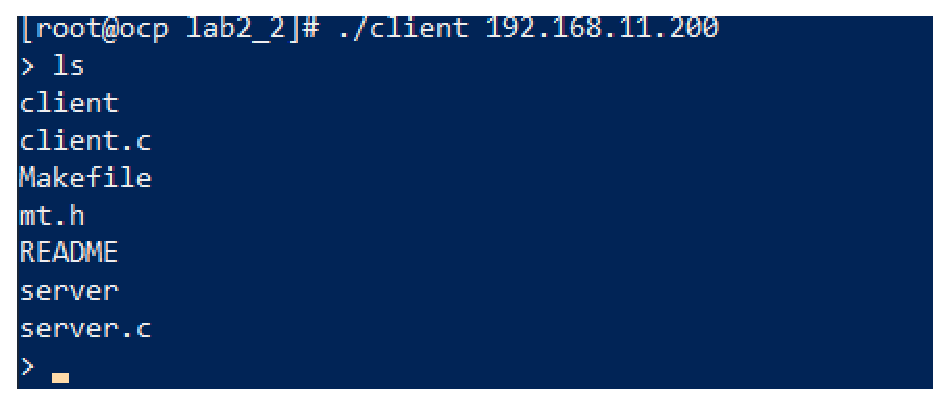
\includegraphics[scale=0.6]{client1}}
\par{客户端2:}
\par\centerline{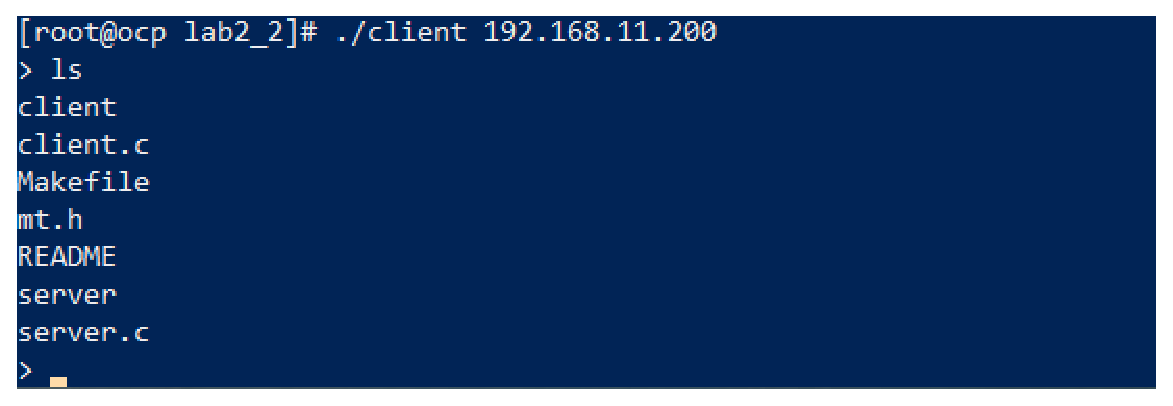
\includegraphics[scale=0.6]{client2}}
\par{从结果图中可以看出,首先本程序的服务器端支持并发,能够同时接受多个客户端的请求。其次,我们执行了ls命令,服务端也争取返回了命令执行的结果,因此该C/S结构程序是有效的。}
\subsubsection{服务端终端:}
\par{服务端:}
\par\centerline{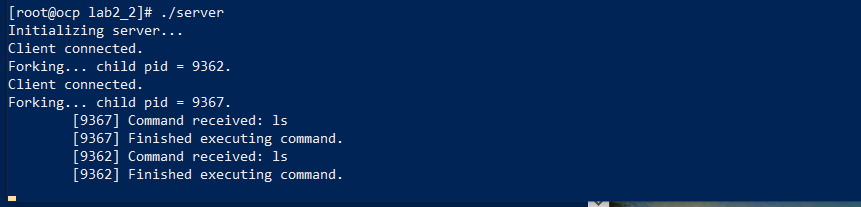
\includegraphics[scale=0.6]{server}}
\par{服务端首先初始化服务器,即配置TCP/IP服务,完成初始化后即可开始接受请求,每来一个客户端请求,都会开辟一个新的子进程来处理请求,同时采用不同的端口分别和客户端进行通信,并且显示进程与具体的执行命令,可以记录log日志。}
\subsection{总结}
\par{通过本次实验,初步了解了Telnet协议的底层原理,并且通过动手实践,实现了一个Telnet程序,能够实现远程主机控制,并且有较好的使用结果。}
\end{document}
